\documentclass[aspectratio=169]{beamer}
% \documentclass{scrartcl}
% \usepackage{beamerarticle}

% TODO: Remove `handout' before presentation

\usepackage{upquote}
\usepackage{minted}
\usepackage{soul}
\usepackage{graphicx}
\usepackage{amssymb}
\usepackage{amsmath}
\usepackage{hyperref}

\usetheme{Hannover}
\setbeamertemplate{navigation symbols}{}

\setlength{\parskip}{1ex}

\title{Programming Paradigms}
\author{\href{https://www.andrewyu.org/}{Runxi Yu}}
\institute{\textit{Colloquium Cognitionis Callidum} 2023}
\date{August 6, 2023}

\begin{document}
\maketitle

\section{Intro}

\begin{frame}{Copyright License}
	\small
	The following applies for everything that I wrote, which is everything other than the XKCD comics:

	Copyright © 2023 Runxi~Yu (\texttt{runxi@andrewyu.org})

	Permission is hereby granted, free of charge, to any person obtaining a copy of this document and associated files (the ``Work''), to deal in the Work without restriction, including without limitation the rights to use, copy, modify, merge, publish, distribute, sublicense, and/or sell copies of the Work, and to permit persons to whom the Work is furnished to do so, subject to the following conditions:

	The above copyright notice and this permission notice shall be included in all copies or substantial portions of the Work.

	The work is provided ``as is'', without warranty of any kind, express or implied, including but not limited to the warranties of merchantability, fitness for a particular purpose and noninfringement. In no event shall the authors or copyright holders be liable for any claim, damages or other liability, whether in an action of contract, tort or otherwise, arising from, out of or in connection with the work or the use or other dealings in the work.
\end{frame}

\begin{frame}{External Copyright}
	This work also includes XKCD comics which are licensed under the Creative Commons Attribution Non-commercial 2.5 license.
\end{frame}

\begin{frame}{Fun fact}
	Me attempting to decide on a topic:
	\begin{itemize}
		\item Epistemology and the limitations of science and formal logic
		\item Elliptic-curve cryptography: Curve25519, Curve448
		\item Memory management: Manual, garbage collection, reference counting, borrow checking, use-after-free, and memory leaks
		\item Liberal feminism and trans-exclusive radical feminism
		\item Cybersecurity: Why school networks are always vulnerable (no)
		\item The federal court system of the United States
		\item \textbf{Programming paradigms}
	\end{itemize}

	Also, \url{https://git.andrewyu.org/andrew/school/ccc.git/plain} has the presentation and related files.
\end{frame}

\begin{frame}{Expected Knowledge}
	This presentation expects a little bit of knowledge in programming. You should know basic operations in at least one general-purpose programming language (no, not HTML).

	You don't have to understand copmilers and interpreter design, or understand a plethora of languages, though the latter may be helpful.

	If you understand and use the Lisp family of languages, or if you have sufficient experience in Haskell using the \texttt{IO} type correctly, you probably don't need to listen to this.
\end{frame}

\begin{frame}{Contents}
	\tableofcontents
\end{frame}

\begin{frame}{Factorials}
	We'll be using the factorial function (classic) as examples.

	Let $n\in\mathbb{N}$,
	\begin{equation*}
		\mathsf{fac}(n) = n! = n\times (n-1)\times (n-2)\times\ldots\times 2\times 1
	\end{equation*}

	\tiny (Yes, math in sans-serif is cringe)
\end{frame}

\begin{frame}{Programming Paradigms?}
	Look at the navigation sidebar.\pause

	\Large\textbf{Why haven't I ever heard of this?}

	\pause\normalsize

	You probably thought that imperative was the only programming paradigm, without actually knowing any others~\ldots

	\pause

	I mean it is quite common
\end{frame}


\section{Imperative}

\begin{frame}[fragile]{Some ``Normal'' C Code}
	\setlength{\parskip}{0ex}
	\small
	\begin{minted}[tabsize=4]{c}
static int seed_with_urandom(void) {
	unsigned int seed;
	int fd;
	fd = open("/dev/urandom", O_RDONLY);
	if (fd >= 0) {
		if (read(fd, &seed, sizeof(seed)) ==
	        		sizeof(seed)) {
			close(fd);
			srand(seed);
			return 1;
		}
		close(fd);
	}
	return 0;
}
	\end{minted}
	\pause
	\textbf{Each statement modifies the program's state.}
\end{frame}

\begin{frame}[fragile]{A Mini Bootloader}
	The following X86 assmebly code, which is part of a master boot record, loads 16 kilobytes of data immediately following the MBR from disk and executes it. X86 assembly is a good example of very imperative programming.
	\begin{minted}[tabsize=4,escapeinside=||]{nasm}
mov ah, 0x02     ; BIOS read disk
mov al, 32       ; 32 sectors
mov ch, 0        ; Cylinder 0
mov cl, 2        ; Sector 2
mov dh, 0        ; Head 0
mov dl, 0x80     ; First hard disk
mov bx, 0x7E00   ; RAM Destination
int 0x13
jc derr
jmp 0x0000:0x7E00
	\end{minted}
\end{frame}

\begin{frame}{The Imperative Paradigm}
	\begin{itemize}
		\item The computer executes statements one-by-one
		\item Each instruction changes the state

			(Which could be memory, CPU registers, etc.)
		\item We may \texttt{jmp}/\texttt{goto} to another instruction
		\item We arrive at a final result from the final state
	\end{itemize}

	\pause But there's a problem with \texttt{goto} \ldots
\end{frame}

\begin{frame}[fragile]{Assembly Control Flows}
	\begin{columns}
		\column{0.5\textwidth}
		\begin{minted}[tabsize=4,escapeinside=||]{nasm}
_start:
	cmp esi, 1
	je .yes
	jmp .no
.yes:
	; do A
	jmp .done
.no:
	; do B
.done:
	; do C
		\end{minted}
		\column{0.5\textwidth}
		\begin{minted}[tabsize=4,escapeinside=||]{c}
if (var == 1) {
	// do A
}
else {
	// do B
}
// do C
		\end{minted}
	\end{columns}
\end{frame}

\begin{frame}{\texttt{goto} Considered Harmful?}
	\begin{figure}
		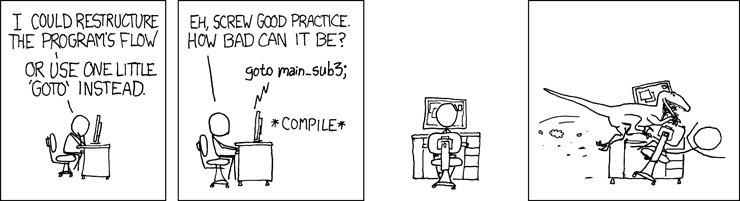
\includegraphics[width=\linewidth]{goto.png}
		\caption{XKCD 292 ``goto'' (CC BY-NC 2.5)}
	\end{figure}
	(\texttt{jmp} and \texttt{goto} are basically the same, and the dinosaur is Goto Dengo in the novel \textit{Cryptonomicon})
\end{frame}

\begin{frame}[fragile]{\texttt{goto} Leads to Spaghetti Code}
	Which of these factorial functions is more readable?
	\begin{columns}
		\column{0.5\textwidth}
		\small
		\begin{minted}[tabsize=4,escapeinside=||]{c}
if (n >= 0)
	goto good;
errno = EINVAL;
return -1;
good:
	int r = 1;
loop:
	if (n > 1)
		goto yes;
	goto end;
yes: 
	r *= n;
	n--;
	goto loop;
end:
	return r;
		\end{minted}
		\column{0.5\textwidth}
		\begin{minted}[tabsize=4,escapeinside=||]{c}
if (n < 0) {
	errno = EINVAL;
	return -1;
}
int r = 1;
for (; n > 1; n--) {
	r *= i;
}
return r;
		\end{minted}
	\end{columns}
\end{frame}

\begin{frame}[fragile]{\textbf{Structured} Imperatives}
	\begin{columns}
		\column{0.5\textwidth}
		\begin{itemize}
			\item Code can be \{grouped\} into blocks.
			\item There are loops!
			\item No more spaghetti \texttt{goto}s.
		\end{itemize}
		\column{0.5\textwidth}
		\small
		\begin{minted}[tabsize=4,escapeinside=||]{c}
int factorial(int n) {
	if (n < 0) {
		errno = EINVAL;
		return -1;
	}
	int r = 1;
	for (; n > 1; n--) {
		r *= i;
	}
	return r;
}
		\end{minted}
	\end{columns}
\end{frame}

\section{Procedural}

\begin{frame}[fragile]{Procedures}
	We could abstract commonly-used procedures into \ldots{} procedures!
	\begin{columns}
		\column{0.5\textwidth}
		\begin{minted}[tabsize=4,escapeinside=||]{c}
char s[] = "Hello";
write(1, s, strlen(s));
write(1, "\n", 1);

char s[] = "Hey there";
write(1, s, strlen(s));
write(1, "\n", 1);
		\end{minted}
		\column{0.5\textwidth}
		\begin{minted}[tabsize=4,escapeinside=||]{c}
void puts(char s[]) {
	write(1, s, strlen(s));
	write(1, "\n", 1);
}

puts("Hello");
puts("Hey there");
		\end{minted}
	\end{columns}
	\medskip
	(Please don't actually use this code which doesn't properly handle errors, but this illustrates the point)
\end{frame}

\begin{frame}[fragile]{Functions}
	We could abstract commonly-used procedures that give us an output into \ldots{} functions!
	\footnotesize
	\begin{columns}
		\column{0.5\textwidth}
		\begin{minted}[tabsize=4,escapeinside=||]{c}
int r, n;

r = 1;
for (n = 5; n > 1; n--) {
	r *= i;
}
printf("%d", r);

r = 1;
for (n = 10; n > 1; n--) {
	r *= i;
}
printf("%d", r);
		\end{minted}
		\column{0.5\textwidth}
		\begin{minted}[tabsize=4,escapeinside=||]{c}
int factorial(int n) {
	if (n < 0) {
		errno = EINVAL;
		return -1;
	}
	int r = 1;
	for (; n > 1; n--) {
		r *= i;
	}
	return r;
}

printf("%d", factorial(5));
printf("%d", factorial(10));
		\end{minted}
	\end{columns}
\end{frame}

\begin{frame}{Why Procedural?}
	Because we don't want to maintain five separate complicated procedures in different parts of the program.

	Also, it saves space, because your object code would only have one copy of the procedure. (But you need to jump between functions with call and return, which might be eversoslightly slower.)
\end{frame}

\section{Object-oriented}

\begin{frame}{Object-oriented???}
	\centering
	I'm not very qualified to talk about this \ldots

	\pause\bfseries\Huge

	Anyone?
\end{frame}

\begin{frame}[fragile]{{\small Small}talk}{A very \st{\tiny small}pure object-oriented language}
	\begin{minted}[tabsize=4]{smalltalk}
Transcript show: 'Hello, world!'.
"Double quotes for comments... strange"
	\end{minted}

	\pause Seriously? \pause Yes.

	\begin{itemize}
		\item Grabs the \texttt{Transcript} object \ldots
		\item Sends a message called \texttt{show} to it \ldots
		\item With the argument \verb|'Hello, world!'|
	\end{itemize}
\end{frame}

\begin{frame}[fragile]{Classes and objects}
	\begin{minted}[tabsize=4]{smalltalk}
"Create a 'Dog' class that accepts 'bark'"
Object subclass: Dog [
	Dog class >> new [
		^ super new
	]

	Dog >> bark [
		Transcript show: 'Woof!'; cr.
	]
]

"Create a new object 'dog' of the class 'Dog'"
dog := Dog new.

"Send the message 'bark' to the object 'dog'"
dog bark.
	\end{minted}
\end{frame}

\begin{frame}{So, what is OOP?}
	Smalltalk as the iconic OOP language:
	\begin{itemize}
		\item Everything is an object, objects are ``instances'' of classes
		\item Classes are descriptions of classes of objects
			\begin{itemize}
				\item Defines the set of messages that its objects respond to
				\item Defines variables contained in classes (not accessible from outside)
			\end{itemize}
		\item Classes can inherit stuff from other classes when being created
	\end{itemize}
\end{frame}

\begin{frame}{Criticism}
	John Ousterhout Scripting, IEEE Computer, March 1998:
	\begin{quote}
		Implementation inheritance causes the same intertwining and brittleness that have been observed when goto statements are overused. As a result, OO systems often suffer from complexity and lack of reuse.
	\end{quote}

	Joe Armstrong:
	\begin{quote}
		The problem with object-oriented languages is they’ve got all this implicit environment that they carry around with them. You wanted a banana but what you got was a gorilla holding the banana and the entire jungle.
	\end{quote}
\end{frame}

\begin{frame}{My Problems with OO}
	\begin{itemize}
		\item Private state that's hidden from the programmer
			
			(The direct opposite of functional programming, sad)
		\item Memory leaks due to references in the private state

			(Though I guess it's better than use-after-free)
		\item Why even mix functions and data?
		\item It's just hard to refactor code with, by experience
	\end{itemize}
\end{frame}

\section{Functional}

\begin{frame}{Functional Programming}
	\begin{itemize}
		\item Programs are representations by applying and composing functions

			Functions are just variables, you can pass them around
		\item Makes it feel closer to pure math
		\item Generally uses higher-order functions, recursion, etc
		\item Functions do not have side effects in a purely functional programming language
	\end{itemize}
\end{frame}

\begin{frame}[fragile]{Haskell Examples}
	\begin{columns}
		\column{0.5\textwidth}
		\begin{minted}[tabsize=4]{haskell}
-- Factorial by recursion
fac 0 = 1
fac n = n * fac (n - 1)

-- Factorial by higher-order
fac n = foldl (*) 1 [1..n]

-- Factorial by cheating :)
fac n = product [1..n]
		\end{minted}
		\column{0.5\textwidth}
		\begin{minted}[tabsize=4,escapeinside=||]{haskell}

		\end{minted}
	\end{columns}
\end{frame}

\begin{frame}{Monads}
	A monad is just a monoid in the category of endofunctors???\\
	\pause
	Monoids, okay, just semigroups with a identity. What's an endofunctor???

	\pause

	\centering
	If anyone here actually know how to explain monads, please do :)

	\pause

	\flushleft
	I only know why they're useful: Abstracting away imperative control flow in a referentially transparent-ish way. (Otherwise you won't be able to actually do anything in pure functional programming.)
\end{frame}

\begin{frame}{Why go through the hassle?}
	Because {\Large mathematics}. (Yeah \ldots)
	\pause
	\begin{itemize}
		\item Easier to formally verify the program to be correct

			Not to be confused with testing
		\item More familiar representation of objects
		\item Better concurrency
		\item Easier to maintain code, encouraging modularity
	\end{itemize}
\end{frame}

\section{Meta-programming}

\begin{frame}{Lisp: Meta-programming}
	What's so great about Lisp? Why is it infrequently used (unless if you use Emacs)?
	\pause
	\begin{itemize}
		\item Lisp is good because it has a very minimal, simple, regular syntax.
		\pause
		\item Lisp is bad because it has a very minimal, simple, regular syntax.
	\end{itemize}
\end{frame}

\begin{frame}[fragile]{Lisp's S-expressions}
	\small
	\begin{minted}{lisp}
(defun main ()
  (print
    (let ((input-table (cl-csv:read-csv #P"tags.csv")))
      (mapcar
        (lambda (row) (let ((new-row (copy-tree row)))
                        (setf (fourth new-row)
                              (mapcar (lambda (s)
                                        (string-trim " " s))
                                      (comma-split (fourth new-row))))
                        (setf (third new-row)
                              (parse-float:parse-float
                                (third new-row)))
                        new-row))
	input-table))))
	\end{minted}
\end{frame}

\begin{frame}{Lisp Macros}
	\begin{itemize}
		\item S-expressions are a simple, uniform syntax
		\item It's very easy to create macros that handle a syntax tree
			
			If you want to, you could create macros that adds control flow that doesn't exist in default Lisp. Maybe introduce a quick notations for Monads while you're at it.
		\item Much better than C preprocessor macros that are literally just string manipulation, much more robust
	\end{itemize}
\end{frame}

\begin{frame}[fragile]{The problem with S-expressions}
	\begin{minted}[breaklines]{lisp}
))))))))))))))))))))))))))))))))))))))))))))))))))))))))))))))))))))))))
))))))))))))))))))))))))))))))))))))))))))))))))))))))))))))))))))))))))
))))))))))))))))))))))))))))))))))))))))))))))))))))))))))))))))))))))))
))))))))))))))))))))))))))))))))))))))))))))))))))))))))))))))))))))))))
))))))))))))))))))))))))))))))))))))))))))))))))))))))))))))))))))))))))
))))))))))))))))))))))))))))))))))))))))))))))))))))))))))))))))))))))))
))))))))))))))))))))))))))))))))))))))))))))))))))))))))))))))))))))))))
))))))))))))))))))))))))))))))))))))))))))))))))))))))))))))))))))))))))
))))))))))))))))))))))))))))))))))))))))))))))))))))))))))))))))))))))))
))))))))))))))))))))))))))))))))))))))))))))))))))))))))))))))))))))))))

(to (the (normal (programmer))) (is this (very (readable))))
(setq readability 1000)
	\end{minted}
\end{frame}

\begin{frame}[fragile]{Example \ldots}
	\tiny
	\begin{minted}{lisp}
(defmacro a (&body b)
  `(progn ,@(mapcar (lambda (c) `(print ,c)) b) ,@(mapcar (lambda (c) `(setq ,c (random 100))) b)))

(defmacro d (e &rest f)
  `(if ,e
       (mapcar (lambda (g) (if (evenp g) (* g g) (* g 3))) ,@f)
       (mapcar #'(lambda (g) (reduce #'* (mapcar #'(lambda (h) (+ h h)) ,@f))) ,@f)))

(defmacro i (j)
  `(mapcar (lambda (k) (if (listp k) (d t k) k)) ,j))

(defun l (m) 
  (mapcar (lambda (n) 
            (mapcar (lambda (o) 
                      (if (and (numberp n) (numberp o)) 
                          (+ n o) 
                          (if (listp n) 
                              (append n (list o)) 
                              (list n o)))) m)) m))

(defun p ()
  (let ((q '(1 2 (3 4) 5 (6 7 8))))
    (a q)
    (d (> (length q) 5) q)
    (l (i q))))

(p)
	\end{minted}
\end{frame}

\begin{frame}
	Which is why modern languages sort of just started copying Lisp concepts into their own language, which works I guess!
\end{frame}

\section{Outro}

\begin{frame}{More?}
	Things I haven't touched upon (I won't say I covered anything in depth today anyways):
	\begin{itemize}
		\item Logic programming
		\item SQL and related declarative languages
		\item Esoteric 
		\item Literate programming
		\item Symbolic programming
	\end{itemize}
\end{frame}

\begin{frame}
	\centering\Huge
	Thanks for listening! Questions?
\end{frame}

\end{document}
